% !TeX encoding = UTF-8
% !TeX spellcheck = pt_BR

%%% PREAMBLE - Do not touch %%%%%%%%%%%%%%%%%%%%%%%%%%%%%%%%%%%%%%%%%%%%%%%%%%%%%%
\documentclass[10pt,twocolumn,letterpaper]{article}
\usepackage[utf8]{inputenc}
\usepackage[portuges,brazil,english]{babel}
\usepackage{model}
\usepackage{times}
\usepackage{epsfig}
\usepackage{graphicx}
\usepackage{amsmath}
\usepackage{amssymb}
\usepackage{color}
\usepackage[pagebackref=true,breaklinks=true,letterpaper=true,colorlinks,bookmarks=false]{hyperref}
%  ABACO -- Conjunto de macros para desenhar o 'abaco
%  Desenho original de Hans Liesenberg
%  Macros de Tomasz Kowaltowski
%  DCC -- IMECC -- UNICAMP
%  Mar,co de 1988  --  Vers~ao 1.0
% Ajustado para LaTeX da SUN -- Mar,co de 1991
% ---------------------------------------------------------
%  Chamada:   \ABACO{d1}{d2}{d3}{d4}{esc}
%             com:  di's -- os quatro d'igitos;
%                   esc  -- fator de escala
% ---------------------------------------------------------
%  DEFINI,C~OES AUXILIARES
% ---------------------------------------------------------
%  Forma o d'igito pequeno (0 ou 1)

\newcommand{\ABACODP}[1]{%
%
\thicklines
%    
\begin{picture}(8,0)
    \ifcase#1{   %  caso 0
       \put(0,0)    {\line(1,0){4}}
       \multiput(5,0)(2,0){2}{\oval(2,4)}}
    \or{         %  caso 1
       \put(2,0)    {\line(1,0){4}}
       \multiput(1,0)(6,0){2}{\oval(2,4)}}
    \fi
\end{picture}
    } % \ABACODP

% Forma o d'igito grande (0 a 4)

\newcommand{\ABACODG}[1]{%
%
\thicklines
%    
\begin{picture}(14,0)
    \ifcase#1{   % caso 0
       \multiput(1,0)(2,0){5}{\oval(2,4)}}
       \put(10,0)   {\line(1,0){4}}
    \or{         % caso 1
       \multiput(1,0)(2,0){4}{\oval(2,4)}}
       \put(8,0)   {\line(1,0){4}}
       \put(13,0)   {\oval(2,4)}
    \or{         % caso 2
       \multiput(1,0)(2,0){3}{\oval(2,4)}
       \put(6,0)   {\line(1,0){4}}
       \multiput(11,0)(2,0){2}{\oval(2,4)}}
    \or{         % caso 3
       \multiput(1,0)(2,0){2}{\oval(2,4)}
       \put(4,0)   {\line(1,0){4}}
       \multiput(9,0)(2,0){3}{\oval(2,4)}}
    \or{         % caso 4
       \put(1,0)  {\oval(2,4)}}
       \put(2,0)   {\line(1,0){4}}
       \multiput(7,0)(2,0){4}{\oval(2,4)}
    \fi
\end{picture}
    } % \ABACODG
       
% Forma um d'igito (0 a 9)

\newcommand{\ABACOD}[1]{%
%
    \ifnum#1>9
       \errmessage{#1: Argumento invalido para ABACO}
    \fi
    \ifnum#1<0
       \errmessage{#1: Argumento invalido para ABACO}
    \fi
%
\begin{picture}(24,0)
%    
    \ifnum#1<5
       \put(16,0) {\ABACODP{0}}
    \else   
       \put(16,0) {\ABACODP{1}}
    \fi
%    
    \ifnum#1<5
       \put(0,0)  {\ABACODG{#1}}
    \else
       \ifcase#1\or \or \or \or
          \or  \put(0,0)  {\ABACODG{0}}
          \or  \put(0,0)  {\ABACODG{1}}
          \or  \put(0,0)  {\ABACODG{2}}
          \or  \put(0,0)  {\ABACODG{3}}
          \or  \put(0,0)  {\ABACODG{4}}
       \fi
    \fi   
\end{picture}
    } % \ABACOD
    
% -------------------------------------------------

%  DEFINI,C~AO PRINCIPAL
    
\newcommand{\ABACO}[5]{%
    \setlength{\unitlength}{#5mm}
%
    \thinlines
%   
\begin{picture}(28,25)
%   
% moldura
%
% externa
%
        \put(0,0)            {\line(0,1){25}}
        \put(0,0)            {\line(1,0){28}}
        \put(28,0)           {\line(0,1){25}}
        \put(0,25)           {\line(1,0){28}}
% interna
        \put(2,2)            {\line(0,1){21}}
        \put(26,2)           {\line(0,1){21}}
        \put(16,2)           {\line(0,1){21}}
        \put(18,2)           {\line(0,1){21}}
        \put(2,2)            {\line(1,0){14}}
%        \put(16,2)           {\line(1,-1){1}}
%        \put(17,1)           {\line(1,1){1}}
        \put(18,2)           {\line(1,0){8}}
        \put(2,23)           {\line(1,0){14}}
%        \put(16,23)          {\line(1,1){1}}
%       \put(17,24)          {\line(1,-1){1}}
        \put(18,23)          {\line(1,0){8}}
%        \put(0,0)            {\line(1,1){2}}
%        \put(0,25)           {\line(1,-1){2}}
%        \put(28,0)           {\line(-1,1){2}}
%        \put(28,25)          {\line(-1,-1){2}}
%
%   
% d'igitos
%
%   
       \put(2,20)  {\ABACOD{#1}}
       \put(2,15)  {\ABACOD{#2}}
       \put(2,10)  {\ABACOD{#3}}
       \put(2,5)   {\ABACOD{#4}}
%      
\end{picture}
    } % \ABACO
    


\cvprfinalcopy % *** Uncomment this line for the final submission
\def\httilde{\mbox{\tt\raisebox{-.5ex}{\symbol{126}}}}
\ifcvprfinal\pagestyle{empty}\fi

\newcommand{\TODO}[1]{TODO: #1}
\newcommand{\CITEONE}[2]{\mbox{#1 \cite{#2}}}
\newcommand{\CITETWO}[3]{\mbox{#1 e #2 \cite{#3}}}
\newcommand{\CITEN}[2]{\mbox{#1 et al. \cite{#2}}}

%%% Report beginning %%%%%%%%%%%%%%%%%%%%%%%%%%%%%%%%%%%%%%%%%%%%%%%%%%%%%%%%%%%%%%
\begin{document}

%%% Title and authors %%%%%%%%%%%%%%%%%%%%%%%%%%%%%%%%%%%%%%%%%%%%%%%%%%%%%%%%%%%%
\title{Identificação de modelos de câmera usando Local Binary Patterns e Sensor Pattern Noise}
\author{Mateus Coelho \thanks{\textbf{Contact}: \tt\small{mateus$\_$coelho@live.com}}}

%%% Abstract %%%%%%%%%%%%%%%%%%%%%%%%%%%%%%%%%%%%%%%%%%%%%%%%%%%%%%%%%%%%%%%%%%%%%
\maketitle
\begin{abstract}

Com a popularização de câmeras digitais quase sempre incluídas em smartphones, há uma preocupação crescente com relação à segurança e à origem de imagens criadas com esses aparelhos. De fato, ao longo da última década a comunidade forense tem desenvolvido vários métodos para identificar modelos de câmeras fotográficas, dos quais dois foram analisados neste projeto: local binary patterns (LBP) e sensor pattern noise (SPN). Aquele é um método conhecido e amplamente utilizado para descrever texturas de imagens e este foi mais recentemente desenvolvido e leva em conta o ruído produzido pelo sensor do aparelho fotográfico para criar features a serem utilizadas no classificador. Então, com essas duas técnicas foram extraídas features que aplicadas em uma regressão logística fornecem um modelo de classificação de câmeras. Para treinar esse modelo foi utilizado um data set com 2750 imagens de 10 modelos de câmeras. O melhor resultado obtido foi empregando o LBP com um score na plataforma Kaggle de 0.531666.

\end{abstract}

%%% Introduction %%%%%%%%%%%%%%%%%%%%%%%%%%%%%%%%%%%%%%%%%%%%%%%%%%%%%%%%%%%%%%%%%
\section{Introdução}

Os avanços nas tecnologias de imagens digitais têm provocado uma revolução no mercado de câmeras fotográficas, já que estas estão a cada dia mais baratas e modernas. Inclusive, a popularização de smartphones contribuiu signifcantemente nessa questão. Cresceu também o número de aplicações que envolvem o uso de imagens digitais, desde uso médico até uso bancário. Porém, com esses avanços tem aumentado também a preocupação com a origem das imagens geradas por esquipamentos digitais, como máquinas fotográficas e scanners. A popularização de softwares de manipulação de imagens é um fator ainda mais crítico nesse aspecto pois permite que pessoas possivelmente desonestas possam utilizá-los para falsificar dados.

Assim, em meio a este cenário, este projeto analisou dois métodos de criar features para alimentar um classificador. O resultado são modelos que tem como entrada uma imagem e como saída o tipo da câmera usada para tirar tal foto.

Esse paper está organizado da seguinte forma: segunda seção mostra soluções já estudadas e presentes na literatura; terceira seção expõe em mais detalhes os métodos utilizados; quarta seção discute os experimentos e resultados obtidos; quinta seção apresenta a conclusão.

%%% Add section %%%%%%%%%%%%%%%%%%%%%%%%%%%%%%%%%%%%%%%%%%%%%%%%%%%%%%%%%%%%%%%%%%
\section{Atividades}

A principal dificuldade em relação ao problema de identificar modelos de câmeras digitais é encontrar features que descrevam com qualidade as imagens. Três métodos de extração de features bastante conhecidos são local binary patterns, wavelet features e sensor pattern recognition.

\CITETWO{Xu}{Shi}{Xu_2012} conseguiu uma acurácia de 98.08\% empregando como features a distribuição resultante do uniform local binary patterns para as três bandas de cor. Além disso usou vetores de erro de predição correspondentes e subbandas da parte diagonal de um wavelet de primeiro nível. Já \CITEN{Wang}{Bo_2009} optou por extrair features de wavelet de alta ordem e features de coocorrência de coeficientes de wavelets. Seu resultado após aplicar Sequential Forward Feature Selection e multi-class SVM foi acurácia de 98\%. Por fim, \CITEN{Filler}{Tomas_2008} estimou e classificou fingerprints (Sensor photo-response non-uniformity) de várias câmeras e modelos diferentes. Para isso extraiu features a partir dos fingerprints que refletem diferenças, por exemplo, no CFA e no sensor de transferência de sinal. A acurácia obtida foi de 90.8\%.

Existem ainda outros jeitos de abordar o problema de identificação de câmeras que se baseiam em etapas específicas do processo de aquisição de uma imagem, mas vários esbarram em problemas como acurácia reduzida para câmeras da mesma marca \cite{Bayram_2005}, transformações geométricas e ataques de ruído.

%%% Add section %%%%%%%%%%%%%%%%%%%%%%%%%%%%%%%%%%%%%%%%%%%%%%%%%%%%%%%%%%%%%%%%%%
\section{Soluções Propostas}

Este paper visa analisar duas maneiras de extrair features de imagens que são local binary patterns e sensor pattern noise. Mais informações sobre eles serão mostrados nas seções abaixo.

\subsection{Local Binary Patterns}

Local binary patterns é tipo de descritor visual amplamente utilizado na área de visão computacional para classificar texturas de imagens digitais. Este método pode ser descrito pelas equações \ref{eq:lbp} e \ref{eq:s}, onde R é o raio de um círculo que representa a vizinhança e P é o número de amostras em volta do círculo. $g_{p}$ e $g_{c}$ são os valores das intensidades no pixels no centro do círculo e em um ponto da amostra do círculo. A diferença desses valores é aplicada na função $s$ e o resultado é computado criando um número binário que representa a comparação do pixel central com seus vizinhos. Para parâmetros $P=8$ e $R=1$, por exemplo, temos a comparação do pixel central com seus 8 vizinhos mais próximos.

\begin{equation}
	\text{LBP}_{P,R} = \sum_{p=0}^{P-1} s(g_{p} - g_{c}) 2^{p}
	\label{eq:lbp}
\end{equation}

\begin{equation}
	s(x) = \begin{cases} 
		1, x \geq 0 \\
		0, x < 0.	
	\end{cases}
	\label{eq:s}
\end{equation}

Computando esse valor para cada pixel de uma imagem tem-se uma distribuição de $2^P$ possíveis valores. O histograma dessa distribuição é, então, o vetor de features que será empregado no classificador. Se a imagem tem três bandas de cor, esse algoritmo deve ser aplicada para a matriz de cada banda.

Uma imagem quando é adquirida pela câmera fotográfica passa por um pipeline de algoritmos, como filtragem e compressão JPEG, que alteram a imagem original com característica localizadas. Segundo \CITETWO{Xu}{Shi}{Xu_2012} este método pode capturar efetivamente essas características geradas pelo pipeline e até certo ponto suprimir a influência do conteúdo da imagem propriamente.

\subsection{Sensor Pattern Noise}

Segundo \CITEN{Lukáš}{Lukas_2006}, na captura de uma imagem por uma câmera fotorgráfica, ela passa por um pipeline de etapas até que o resultado final seja obtido. Algumas etapas são conversão de photons para voltagens, passagem pelas lentes, aplicação de um filtro antialiasing, vetor de filtro de cor etc. Ao longo desse processo ruído introduzido. Este pode ser no final das contas dividido em duas parcelas: FPN e PRNU. O  PRNU (photo-response nonuniformity noise) é parte dominante e quando obtido pode ser utilizado para especificar uma câmera específica. Esse ruído é considerado como a principal parte do fingerprint ("digital") de uma câmera.

Uma aproximação do PRNU pode ser obtido tirando a média do ruído de várias imagens. O ruído de uma imagem é calculado simplesmente subtraindo a imagem original do resultado de um filtro de redução de ruído aplicado na imagem original. Para que a aproximação seja boa, devem ser utilizadas no mínimo 50 ruídos de imagens. No caso desse trabalho, foram utilizadas 50 imagens com um filtro de redução de ruído a base de wavelets com as características presentes na tabela \ref{tab:filtro}. As imagens \ref{fig:ruido} e \ref{fig:ruidom} mostram, respectivamente o ruído de uma imagem e o ruído médio de 50 imagens retiradas do data set do trabalho.

Com os fingerprints em mãos, existem várias maneiras de retirar features para relacionar o ruído médio com o ruído de cada imagem.

\begin{table}[]
\centering
\caption{}
\label{tab:filtro}
\begin{tabular}{|c|c|}
\hline
\multicolumn{2}{|c|}{Filtro de redução de ruído wavelet} \\ \hline
Sigma                        & 0.019                     \\ \hline
Wavelet                      & 8-tap Daubechies QMF      \\ \hline
Níveis de decomposição       & 4                         \\ \hline
\end{tabular}
\end{table}

\begin{figure}
\begin{center}
	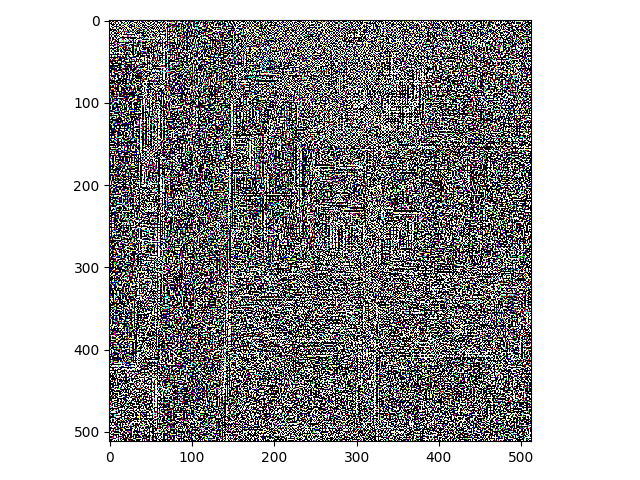
\includegraphics[width=0.99\columnwidth]{pics/ruido.png}
	\caption{Ruído de uma imagem, obtida pela subtração da original pela original filtrada
	\label{fig:ruido}}   
\end{center} 
\end{figure}  

\begin{figure}
\begin{center}
	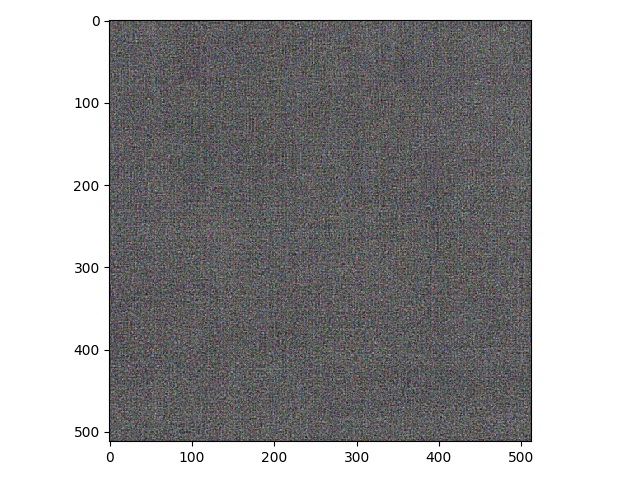
\includegraphics[width=0.99\columnwidth]{pics/ruido_medio.png}
	\caption{Ruído médio de 50 imagens.
	\label{fig:ruidom}}   
\end{center} 
\end{figure}  

%\begin{figure}
%\begin{center}
%	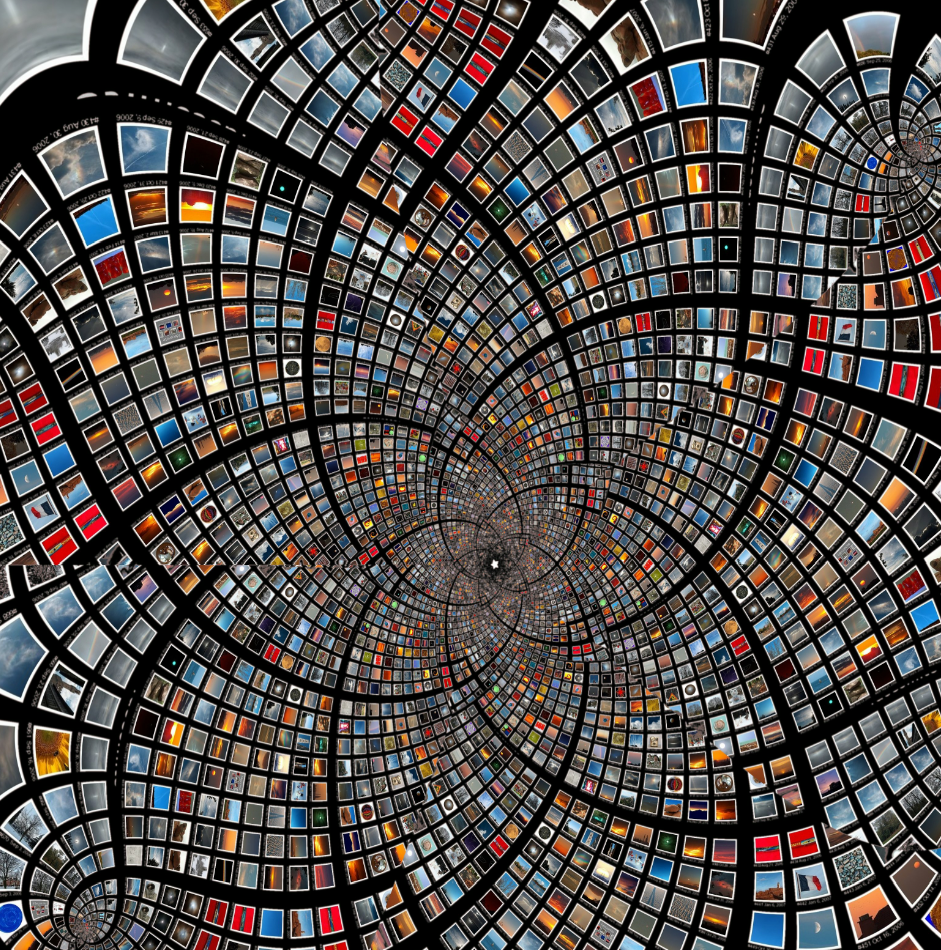
\includegraphics[width=0.99\columnwidth]{pics/example-figure}
%	\caption{A figure example spanning one column only.\label{fig:label}}   
%\end{center} 
%\end{figure}  

\section{Experimentos e Discussão}


%Example of a figure spanning two columns. 
%\begin{figure*}
%\begin{center}
%	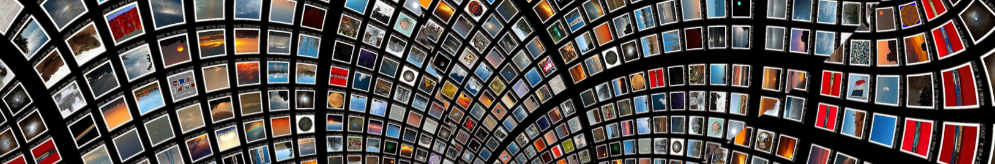
\includegraphics[width=0.99\textwidth]{pics/example-figure-spanned}
%	\caption{A figure example spanning two columns.\label{fig:label2}}   
%\end{center} 
%\end{figure*}
%
%Example of a table spanning only one column: 
%
%\begin{table}
%\begin{center}
%\begin{tabular}{l*{6}{c}r}
%Team              & P & W & D & L & F  & A & Pts \\
%\hline
%Manchester United & 6 & 4 & 0 & 2 & 10 & 5 & 12  \\
%Celtic            & 6 & 3 & 0 & 3 &  8 & 9 &  9  \\
%Benfica           & 6 & 2 & 1 & 3 &  7 & 8 &  7  \\
%FC Copenhagen     & 6 & 2 & 1 & 2 &  5 & 8 &  7  \\
%\end{tabular}
%\end{center}
%\end{table}
%
%Example of a table spanning two columns: 
%
%\begin{table*}
%\begin{center}
%    \begin{tabular}{ | l | l | l | p{8cm} |}
%    \hline
%    Day & Min Temp & Max Temp & Summary \\ \hline
%    Monday & 11C & 22C & A clear day with lots of sunshine.  
%    However, the strong breeze will bring down the temperatures. \\ \hline
%    Tuesday & 9C & 19C & Cloudy with rain, across many northern regions. Clear spells
%    across most of Scotland and Northern Ireland,
%    but rain reaching the far northwest. \\ \hline
%    Wednesday & 10C & 21C & Rain will still linger for the morning.
%    Conditions will improve by early afternoon and continue
%    throughout the evening. \\
%    \hline
%    \end{tabular}
%\end{center}    
%\end{table*}

%%% Add section %%%%%%%%%%%%%%%%%%%%%%%%%%%%%%%%%%%%%%%%%%%%%%%%%%%%%%%%%%%%%%%%%%
\section{Conclusões e Trabalho Futuro}



%%% References %%%%%%%%%%%%%%%%%%%%%%%%%%%%%%%%%%%%%%%%%%%%%%%%%%%%%%%%%%%%%%%%%%%
{\small
\bibliographystyle{unsrt}
\bibliography{refs}
}

\end{document}